\section{QR Decomposition Implementation}

\subsection{CPU}

The standard algorithm for the QR decomposition involves successive Householder transformations \cite[Sect. 2.10.4]{numericalrecipes}. To implement QR decomposition on the CPU, we followed the outline of the algorithm in \cite[Sect. 2.10]{numericalrecipes} almost exactly. In the book's implementation, the Householder algorithm runs on all columns except for the last one. 

We modified the implementation such that the last column is also transformed with the Householder method. By doing this we do not have to handle a special case separately, as the book does, at the end of the algorithm. Our implementation of the algorithm can be seen in listing \ref{lst:qr_decomposition_cpu} in appendix A. 

We have a limited understanding of the underlying math behind QR decomposition, but the general flow of the algorithm is as follows:

\begin{enumerate}
    \item Each column of the matrix is considered one at a time. In iteration k, only elements from the k$_{th}$ element and below are considered. 
    \item For numerical stability purposes all elements will temporarily be scaled down by the maximal entry of the column. 
    \item If all the entries of a column are zero, then the matrix is determined to be singular. 
    \item The diagonal length of the hyperplane with k dimensions is determined by calculating the square root of the sum of the squares of the each entry of the k$_{th}$ column. 
    \item The inner product of the remaining square matrix with dimension k is computed to transform itself. 

\end{enumerate}

As seen in figure \ref{fig:qr_cpu_gpu_sc}, the CPU implementation of QR decomposition has a slope of $\sim 3$, meaning it is similar in time complexity to matrix multiplication. The key difference, however, is that QR decomposition is a lot harder to parallelize, since each iteration of the algorithm depends on the previous.

\begin{figure}[h]
  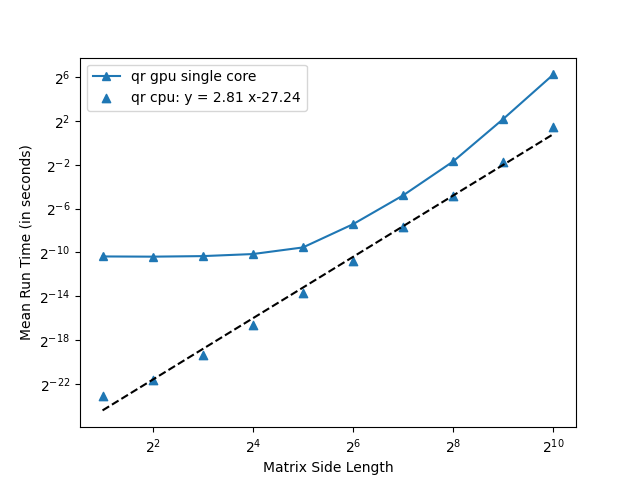
\includegraphics[width=.7\textwidth]{SavedBenchmarksAndDiagrams/Machine 2/QR/GPU SC.png}
  \centering
  \caption{QR: CPU Benchmark and GPU Single Core}
  \label{fig:qr_cpu_gpu_sc}
\end{figure}

We tested the correctness of this algorithm, by recomposing matrix $\mathbf{Q}$ and $\mathbf{R}$ back to the input matrix $\mathbf{A}$.

\subsection{GPU} 

\subsubsection{Single Core}
As with our other single core implementations, the single core implementation for our QR-decomposition is essentially the same as the CPU implementation, although it runs in a kernel with a grid size and block size of one. Our implementation can be seen in listing \ref{lst:qr_gpu_singlecore} in appendix A.

As seen in figure \ref{fig:qr_cpu_gpu_sc}, the single core implementation is constant in the beginning, due to the overhead of allocating memory on the GPU, and then grows similarly to the CPU implementation, once the running time exceeds the overhead. At the end, the slope seems to grow steeper, most likely due to the large amount of floats having to be copied back and forth.

\subsubsection{Parallel Reduction}

To optimize the performance of QR decomposition with GPU accelerated code, we firstly factored out the parts that can run independently. This includes scaling every element of a column by a factor and subtracting a certain value from every element of a column. Each block is responsible for a subset of the column, and each thread is then further responsible for a subset of that subset.

A more interesting problem to solve in parallel is what we have classified reduction algorithms. Reduction algorithms are defined as computing an accumulation of elements by some associative operation. In our case we had to find the maximal absolute element of a column as well as finding the sum of a column. The algorithm we wrote was inspired by \cite{parallelreduction}. The algorithm works by operating on pairs of elements in a tree-like structure until only one element is left, as seen in figure \ref{fig:parallel reduction}. 

\begin{figure}[ht]
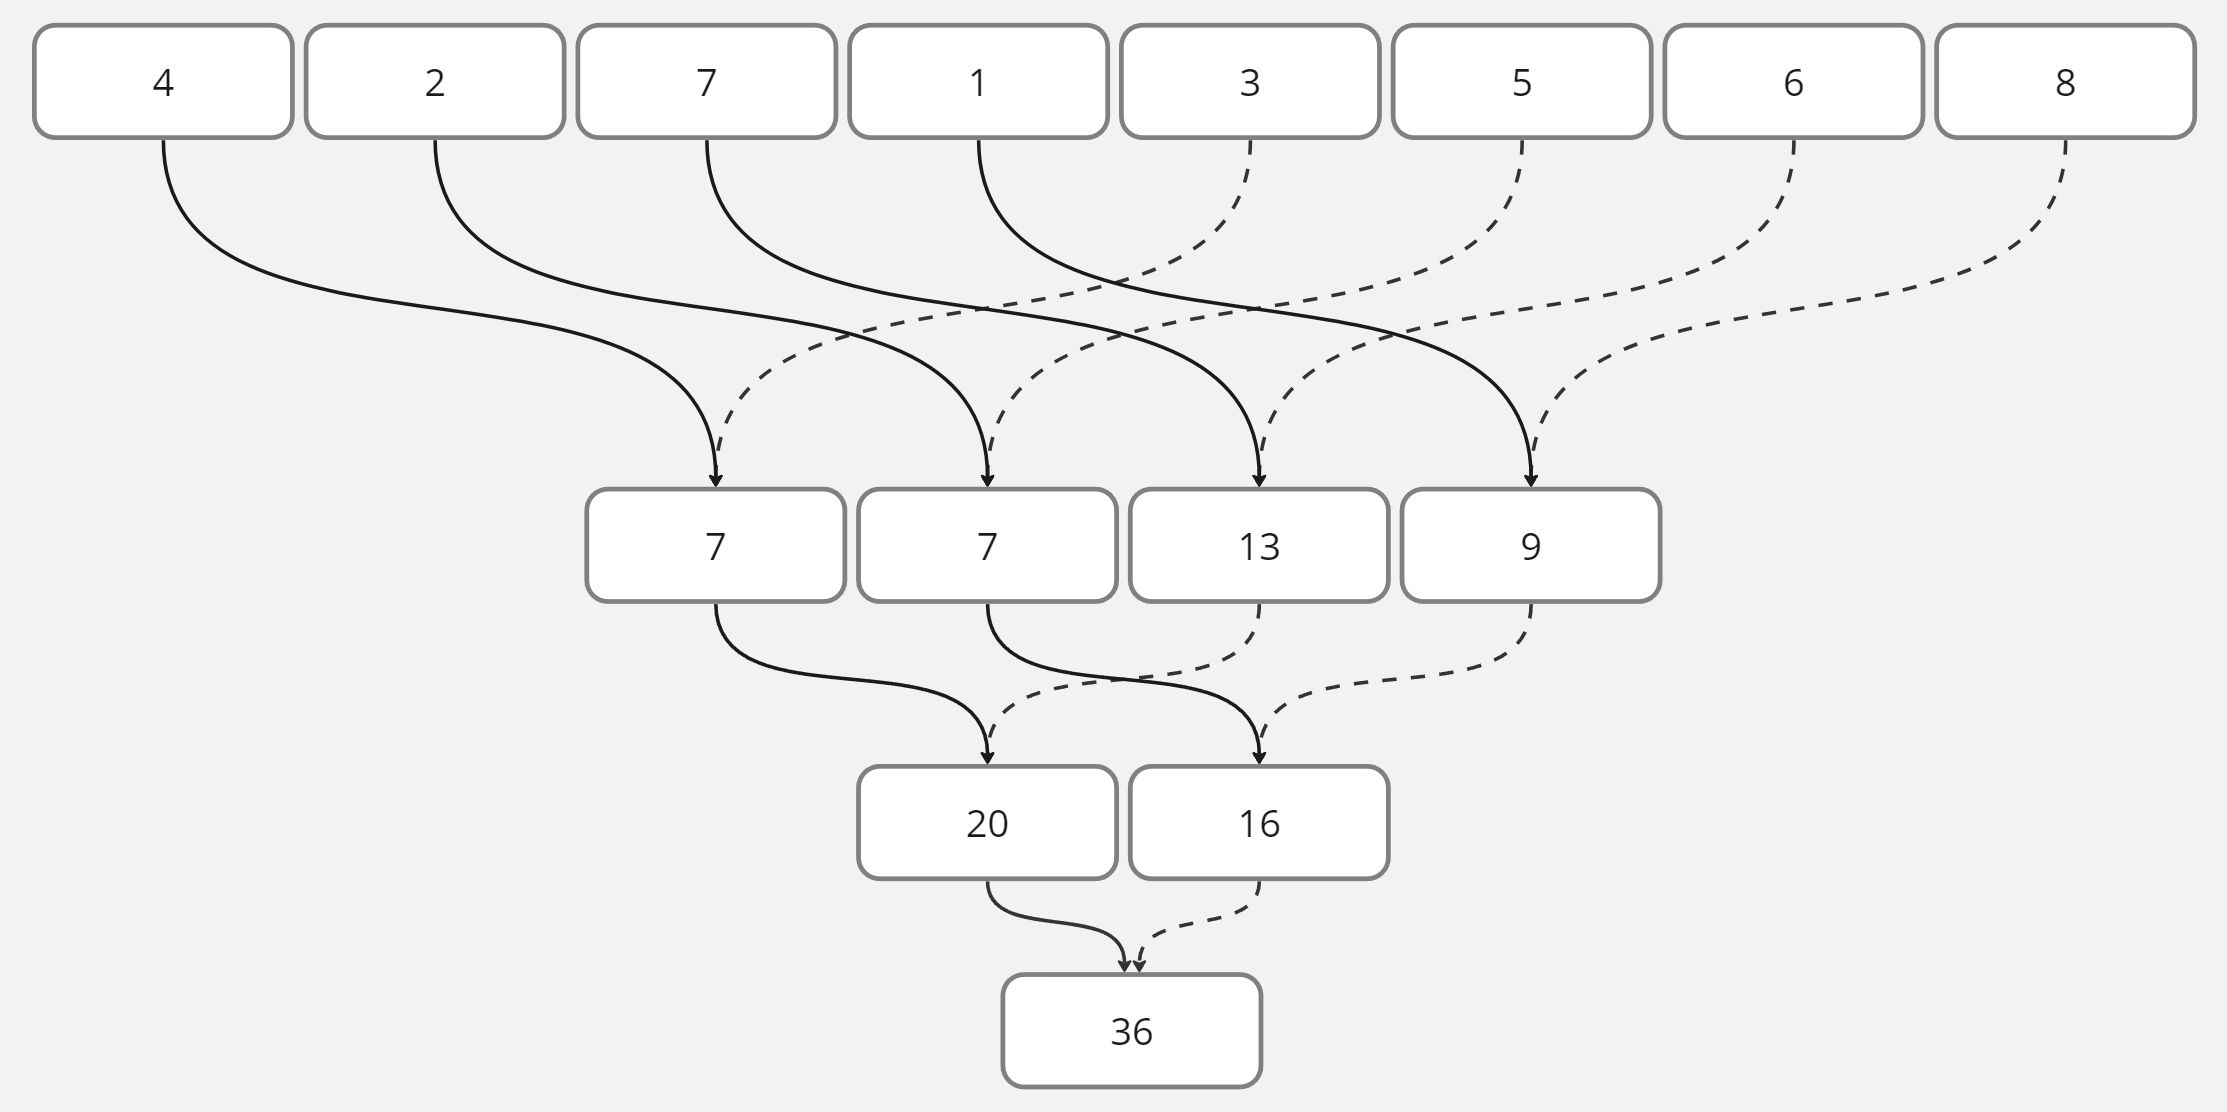
\includegraphics[width=\textwidth]{Documents/Report/Figures/parallel_sum.png}
\caption{Example of summation by parallel reduction.}
\label{fig:parallel reduction}
\end{figure}

Our implementation can be seen in the code below. Please note that our algorithm is generalized such that we can pass any associative function pointer as the reducer.

The algorithm works by distributing the responsibility of each entry in the array to a thread. The $split\_index$ variable keeps track of the middle of the remaining elements to be paired up. This variable also acts as an offset, to calculate which element a given entry should be paired up with. On each iteration $element_i$ is paired up with $element_{i + split\_index}$ and stored in $element_i$. After each iteration, the $split\_index$ is halved. After the final iteration the parallel reduction result is stored at index 0. To prevent accessing out of bounds, we assert that $i < split\_index$. To prevent race conditions, all threads are synchronized before starting the next iteration. 

\begin{lstlisting}[language=C, caption={Parallel Reduction}, label={lst:parallel_reduce}]
typedef float (*reducer_t)(float, float);

__device__ void cuda_parallel_reduction(
    float *cache, int cache_index, reducer_t reduce) {
    int split_index = blockDim.x;
    while (split_index != 0) {
        split_index /= 2;
        if (cache_index < split_index)
            cache[cache_index] =
                reduce(cache[cache_index], cache[cache_index + split_index]);

        __syncthreads();
    }
}
\end{lstlisting}

In our final implementation of a GPU QR decomposition, we utilize a CPU runner responsible for launching kernels. Each kernel is launched with an appropriate amount of threads and blocks depending on the work required. Each column must still sequentially go through the Householder method, thus preventing us from running the algorithm completely in parallel. This runner is also responsible for allocating, copying and freeing memory related to the GPU. 

As seen in figure \ref{fig:qr_parallel}, the parallel max implementation is quite a bit slower than the single core implementation for almost every size. At this point we thought to measure the performance impact of launching multiple kernels. This implementation launches multiple kernels pr. column, so we thought it might be a significant contributing factor to this performance decrease. This hypothesis was confirmed, as seen in the GPU diagnostic back in figure \ref{fig:diagnostic_benchmark}.


\begin{figure}[h]
  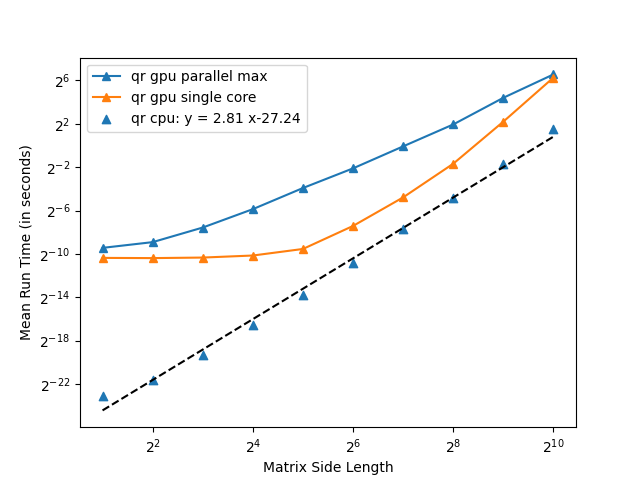
\includegraphics[width=\textwidth]{SavedBenchmarksAndDiagrams/Machine 2/QR/GPU Parallel Max.png}
  \centering
  \caption{QR: All benchmarks}
  \label{fig:qr_parallel}
\end{figure}


A major performance disadvantage to the QR decomposition algorithm is that it must iterate through columns. Column elements are not sequentially aligned in memory, so many cache misses will occur. This causes the machine to fill its cache with data that will not be used immediately for computation, leading to more time spent fetching relevant data. 